\section{Hash functions over MPC}
%\subsection{MPC-friendly hash functions}
Traditional hash functions such as \KECCAK operate over binary fields to enable efficient implementations in both hardware and software on a wide range of platforms.
However, they lead to poor performance when employed within advanced cryptographic protocols such as MPC.
This is mainly due to the fact that traditional schemes are designed to minimize their overall gate count without minimizing specifically nonlinear gates\footnote{They are actually symmetric designs that aim at minimizing the number of nonlinear gates for efficient software masked implementations against side-channel attacks, see for instance~\cite{fse-2014-27573}.} which require communication between parties in an MPC setting, unlike linear gates that can be computed locally.
The overload induced by these communications is such that it can constitute the bottleneck in MPC protocols, as highlighted by an attempt to thresholdize PQC signatures schemes~\cite{sharing_luov19}.
In response, new primitives with design constraints finely tuned for advanced cryptographic protocols have emerged, known as \textit{arithmetization-oriented} primitives.
They usually operate over $\mathbb{F}_p$ with $p$ prime, making them natively compatible with linear secret sharing schemes, and rely on multiplications for nonlinear operations.
Among them, \Poseidon~\cite{poseidon} has found its place into many Ethereum applications thanks to its efficiency in verifiable computing and its successor \PoseidonTwo~\cite{poseidon2} is currently being considered for Ethereum protocols that rely on zero-knowledge proofs\footnote{\url{https://www.poseidon-initiative.info/}}.
\subsection{The Poseidon2 family of hash functions}
%Because the generalized \XMSS scheme introduced in~\cite{} has been instantiated with \PoseidonTwo for benchmarking purposes, we will use this hash function for 
%\paragraph{Poseidon2}
\paragraph{Overview.}
\PoseidonTwo is built upon the \PoseidonTwoPi permutation operating over $\mathbb{F}_p^t$ with $p > 2^{30}$ prime and $t \in \{2,3,4,8,12,16,20,24\}$. %such that $t = c + r$ where $c$ and $r$ refer to the capacity and rate of the sponge construction, respectively. %being Substitution-Permutation Networks (SPN) based on the HADES design strategy.
The permutation is meant to be combined with either a compression function or a sponge construction to build a hash function.
\PoseidonTwoPi is based on the HADES design strategy which makes a distinction between external and internal rounds.
Internal rounds (also called partial rounds) apply the nonlinear layer to only a part of the state, usually a single element, whereas external rounds (also called full rounds) process all elements in the same way.
More precisely, \PoseidonTwoPi processes an internal state $x = (x_0,\cdots,x_{t-1}) \in \mathbb{F}_p^t$ as follows:
\begin{align*}
 \mathsf{Poseidon2}^{\pi}(x) = \mathcal{E}_{R_F-1} \circ \cdots \circ \mathcal{E}_{R_F/2} \circ \mathcal{I}_{R_P-1} \circ \cdots \circ \mathcal{I}_{0}\circ \mathcal{E}_{R_F/2-1} \circ \cdots \circ \mathcal{E}_{0}(M_{\mathcal{E}} \cdot x) \,
\end{align*}
where $\mathcal{E}$ and $\mathcal{I}$ refer to external and internal round functions iterated for $R_F$ and $R_P$ rounds, respectively.
Note that a linear layer is applied before running the first external round, which differs from the original \PoseidonPi design.
The external/full round function is defined by:
\begin{align*}
 \mathcal{E}(x) = M_{\mathcal{E}} \cdot \Big(\big(x_0+c_0^{(i)}\big)^d,\cdots,\big(x_{t-1}+c_{t-1}^{(i)}\big)^d\Big) \,
\end{align*}
where $d \geq 3$ is the smallest integer such that gcd$(d,p-1) = 1$, $M_{\mathcal{E}}$ is a $t \times t$ maximum distance separable (MDS) matrix and $c_j^{(i)}$ is the $j$-th round constant for the $i$-th external round.
The internal/partial round function is defined by:
\begin{align*}
 \mathcal{I}(x) = M_{\mathcal{I}} \cdot \Big(\big(x_0+\hat{c}_0^{(i)}\big)^d,x_1,\cdots,x_{t-1}\Big) \,
\end{align*}
where $d \geq 3$ as before, $M_{\mathcal{I}}$ is a $t \times t$ MDS matrix and $\hat{c}_0^{(i)}$ is the round constant for the $i$-th internal round.


\paragraph{Efficient instantiations for hash-based signatures over MPC.}
Since \PoseidonTwo is a generic construction, all instantiations will most likely not provide the same level of MPC-friendliness.
Because all operations but exponentiations can be computed locally in an MPC setting, one should aim at minimizing the $d$ parameter as it would result in fewer multiplications.
From a permutation-only perspective, one would also be tempted to minimize $t$ and $R = R_F + R_P$ parameters  as the amount of exponentiations is directly derived from them.
However, at the hash function level, the optimal parameter selection depends on the input size to be processed. Indeed for large inputs that require a sponge mode as the underlying construction, having a large rate would allow to absorb more data per permutation, and eventually leading to fewer calls and fewer exponentiations in the end.
In the case of hash-based signatures, most hash calls process small inputs to compute either hash chains from secret keys or nodes in the Merkle tree, with the exception of leafs which are obtained by hashing multiple public keys.
This is why the generalized \XMSS scheme from~\cite{cryptoeprint:2025/055} instantiates \PoseidonTwo with the compression mode for chain and tree hashing, whereas it uses the sponge mode for leaf hashing.
%For hash-based signatures over MPC however, one can disregard the specific case of tree hashing: since all inputs are public it is possible to recombine the shared values together to run the calculations in a non-distributed manner.
%Therefore, we focus solely on instantiations based on the compression mode.
More specifically, their instantiations use a 31-bit prime field for efficient SNARK-based aggregation with $t = 16$ and $t = 24$ for chain and leaf hashing, respectively.
We will hence focus on these parameters in the rest of this document.
%Table~\ref{tab:poseidon2_inst31} lists the relevant \PoseidonTwoPi parameters for two such primes, namely Mersenne31 and BabyBear, which enable highly efficient implementation techniques.
%The remaining parameters of interest, namely $d$ and $R = R_F + R_P$, depend on the value of $p$ as detailed in 

\subsection{Performance assessment}
\paragraph{Hash chains over MPC.}
Benchmarking MPC protocols is challenging as their efficiency not only depends on the underlying cryptographic primitives but also on the security model, number of participants and network conditions.
Because only nonlinear operations require communication between participants, the number of multiplications provides a good performance indicator.
If a multiplication usually requires one communication round along with some precomputed data (\textit{i.e.}, Beaver triples), in the case of exponentiation it is possible to lower the number of communication rounds at the cost of more precomputation.
Therefore, the technique employed to compute $x^d$ has a significant impact on performance.
To estimate the number of communication rounds required for \PoseidonTwoPi over 31-bit prime fields, we used the MP-SPDZ framework~\cite{mp-spdz}\footnote{\url{https://github.com/data61/MP-SPDZ}} with the MASCOT protocol~\cite{mascot} which provides active security.
The \PoseidonTwoPi implementation, meant to be compiled by MP-SPDZ, is available at \url{https://github.com/ObolNetwork/pqdv/blob/main/poseidon2.mpc}.
We considered three different 31-bit prime fields which enable highly efficient implementation techniques, namely Mersenne31, KoalaBear and BabyBear.
As reported in Table~\ref{tab:poseidon2_inst31}, even though the KoalaBear prime field leads to the highest number of rounds, it is actually more MPC-friendly\footnote{KoalaBear and BabyBear primes also show advantages over Mersenne31 when it comes to SNARKS thanks to their two-adic multiplactive subgroups for Cooley-Tukey NTTs.} than the two others thanks to its minimal $d$ value.
Having now an idea on the number of communication rounds per permutation, it is necessary to evaluate how many permutation calls are needed to sign a message (it actually also matters for DKG, but we will assume it is not an issue at this stage as it suffers less timing constraints).
To do so, we rely on the \XMSS instantiations with \PoseidonTwo from~\cite{cryptoeprint:2025/055} and use a script developped by the authors\footnote{\url{https://github.com/b-wagn/hashsig-parameters}} to calculate the number of permutation calls to sign a message in the average case.
According to the instantiations considered in Table~\ref{tab:xmss_poseidon2_permcalls}, on average, the number of permutation calls for hash chains is at least 78.
While at first glance it seems that $78 \cdot 30 = 2\,340$ communication rounds are required to generate a signature, a single communication round can actually be used for multiple multiplications as long as they do not depend on each other.
In the case of hash-based signature, since each chunk is processed independently, it is possible to leverage these parallelization capabilities at the chunk level.
Still, in the worst case where a $w$-bit chunk has value $2^w-1$, then at least $(2^w-1) \cdot 30$ rounds will be needed anyway due to the nature of hash chains.
Like all hash-based signatures schemes, instantiations with low $w$ parameter (typically $w \in \{1,2\}$) are the most MPC-friendly as they require fewer hash calls.
On the other hand, they lead to very a large signature size and will likely not be considered for deployment on the Ethereum beacon chain for this reason.
Among the instantiations listed in Table~\ref{tab:xmss_poseidon2_permcalls}, the ones with $w=4$ seem the most promising as they provide a nice trade-off between signature size and running time.
By leveraging parallelization capabilities, it would require $16 \cdot 30 = 480$ communication rounds to generate a signature, assuming KoalaBear prime field.

\renewcommand\arraystretch{1.25}
\begin{table}[t]
	\centering
	\begin{tabular}{cccccccc}
		\toprule
    		\textbf{Prime} $p$ & \multicolumn{4}{c}{\textbf{Parameters}} & \textbf{Sbox impl.} & \multicolumn{2}{c}{\textbf{MPC cost metrics}}\\
    		 & {$t$} & {$d$} & {$R_F$} & {$R_P$} & & (triples, squares) & com. rounds\\
    		\midrule
   
    		& 16 &  & & 20 &  & $(148, 148)$ & 30 \\
    		%\cmidrule[0.4pt]{2-8}
    		\multirow{-2}{*}{$2^{31}-2^{24}+1$} & 24 & \multirow{-2}{*}{3} & \multirow{-2}{*}{8} & 23 &  \multirow{-2}{*}{$x^3$} & $(215, 215)$ & 33\\
    		\midrule
    		& 16 &  &  & 14 & & $(426, 0)$ & 66 \\
    		%\cmidrule[0.4pt]{2-8}
    		\multirow{-2}{*}{$2^{31}-1$} & 24 & \multirow{-2}{*}{5} & \multirow{-2}{*}{8} & 22 &  \multirow{-2}{*}{$(x^2)^2 \cdot x$} & $(624, 0)$ & 90\\
    		\midrule
    		& 16 & & & 13 &  & $(423, 141)$ & 63\\
    		\multirow{-2}{*}{$2^{31}-2^{27} + 1$}  & 24  & \multirow{-2}{*}{7} & \multirow{-2}{*}{8} & 21 &  \multirow{-2}{*}{$(x^2)^3 \cdot x$ }  & $(639, 213)$  & 87\\
    		\bottomrule
	\end{tabular}
	\caption{\PoseidonTwoPi parameters for 31-bit prime fields.\label{tab:poseidon2_inst31}}
\end{table}

%\subsection{Secure multiplication}

\renewcommand\arraystretch{1.25}
\begin{table}[h]
	\centering
  	%\resizebox{\textwidth}{!}{  
	\begin{tabular}{cccccc}
		\toprule
    		\textbf{Encoding} & \multicolumn{2}{c}{\textbf{Parameters}} & \multicolumn{2}{c}{\textbf{Sig. size} (KiB)}  & \textbf{Perm. calls} \\
    		 & {$w$} & chunks  & $L=2^{18}$ & $ L=2^{20}$ & (average case)   \\
    		\midrule
	     &  1 & 163 & 4.97 & 5.03 & 81    \\
	     &  2 & 82  & 2.75 & 2.81 & 123 \\
	     &  4 & 42  & 1.66 & 1.72 & 303 \\
	 \multirow{-4}{*}{W}  & 8 & 22 & 1.11 & 1.34 & 2676 \\
	 \midrule
 	   &  1 & 155 & 4.75 & 4.81 & 78   \\
	   &  2 & 78  & 2.65 & 2.7  & 117  \\
	   &  4 & 39  & 1.58 & 1.64 & 293  \\
	 \multirow{-4}{*}{TSW ($\delta = 1$)}  &  8 & 20 & 1.06 & 1.27 & 2550  \\
	\hline
	\end{tabular}
	%}
	\caption{Generalized \XMSS instantiations with \PoseidonTwo over a 31-bit prime field. The reported number of permutation calls only considers hash chains during signature generation. For signature sizes, we consider two different leaf numbers, namely $L \in \{2^{18}, 2^{20}\}$. Regarding encodings, we refer to the original publication~\cite{cryptoeprint:2025/055} for more details.\label{tab:xmss_poseidon2_permcalls}}
\end{table}

\newpage

\paragraph{Precomputed hash chains.}
As mentioned in the previous section, another alternative would be to precompute all hash chain intermediate values, for each secret key and for every possible chunk.
Therefore the memory usage would be $L \cdot (2^w-1) \cdot \#\mathsf{chunks}$ digests where $L$ refers to the number of leafs in the Merkle tree.
For the instantiations reported in Table~\ref{tab:xmss_poseidon2_permcalls}, where hashs are composed of either 7 or 8 field elements, it requires $\approx 2, 2, 4, 40$ GiB for $L= 2^{18}$ and $w = 1, 2, 4, 8$ respectively.

%\renewcommand\arraystretch{1.25}
%\begin{table}[htbp]
%	\centering
%  	\resizebox{\textwidth}{!}{  
%	\begin{tabular}{cccccccc}
%		\toprule
%    		\textbf{Encoding} & \multicolumn{2}{c}{\textbf{Parameters}} & \multicolumn{2}{c}{\textbf{Sig. size} (KiB)}  & \textbf{Perm. calls} & \multicolumn{2}{c}{\textbf{Precomp. cost} (GiB)} \\
%    		 & {$w$} & chunks  & $L=2^{18}$ & $ L=2^{20}$ & (average case) &  $L=2^{18}$ & $ L=2^{20}$  \\
%    		\midrule
%	     &  1 & 163 & 4.97 & 5.03 & 81  & 2.22 & 8.91  \\
%	     &  2 & 82  & 2.75 & 2.81 & 123 & 2.24 & 8.96  \\
%	     &  4 & 42  & 1.66 & 1.72 & 303 & 4.59 & 18.37 \\
%	 \multirow{-4}{*}{W}  & 8 & 22 & 1.11 & 1.34 & 2676 & 41.91 & 176 \\
%	 \midrule
% 	   &  1 & 155 & 4.75 & 4.81 & 78   & 2.11 & 8.47 \\
%	   &  2 & 78  & 2.65 & 2.7  & 117  & 2.13 & 8.5 \\
%	   &  4 & 39  & 1.58 & 1.64 & 293  & 4.26 & 17.06 \\
%	 \multirow{-4}{*}{TSW ($\delta = 1$)}  &  8 & 20 & 1.06 & 1.27 & 2550 & 40 & 160 \\
%	\hline
%	\end{tabular}
%	}
%	\caption{Generalized \XMSS instantiations with \PoseidonTwo over a 31-bit prime field. The reported number of permutation calls only considers hash chains during signature generation.
%	 Regarding encodings, we refer to the original publication~\cite{cryptoeprint:2025/055} for more details.}
%\end{table}


\begin{figure}
\centering
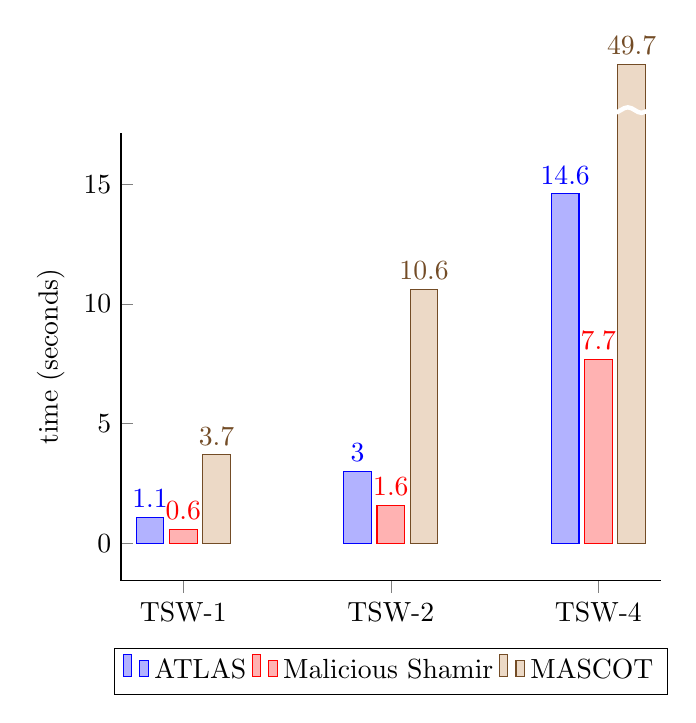
\begin{tikzpicture}
\begin{axis}[
    ybar,
    ymax=15,
    enlargelimits=0.15,
    legend style={at={(0.5,-0.15)},
      anchor=north,legend columns=-1},
    ylabel={time (seconds)},
    symbolic x coords={TSW-1,TSW-2,TSW-4},
    xtick=data,
    restrict y to domain*=0:20, % Cut values off at 20
    visualization depends on=rawy\as\rawy, % Save the unclipped values
    after end axis/.code={ % Draw line indicating break
            \draw [ultra thick, white, decoration={snake, amplitude=1pt}, decorate] (rel axis cs:0,1.05) -- (rel axis cs:1,1.05);
        },
    nodes near coords={%
            \pgfmathprintnumber{\rawy}% Print unclipped values
        },
    nodes near coords align={vertical},
    axis lines*=left,
    clip=false
    ]
\addplot coordinates {(TSW-1,1.1) (TSW-2,3) (TSW-4,14.6)};
\addplot coordinates {(TSW-1,0.6) (TSW-2,1.6) (TSW-4,7.7)};
\addplot coordinates {(TSW-1,3.7) (TSW-2,10.6) (TSW-4,49.7)};
\legend{ATLAS, Malicious Shamir, MASCOT}
\end{axis}
\end{tikzpicture}
\caption{Benchmark results for hash chains calculations over MPC (online phase only) to sign a single message. Timing results are averaged over 10 runs in a network with 30ms delay.}
\end{figure}


\begin{figure}
\centering
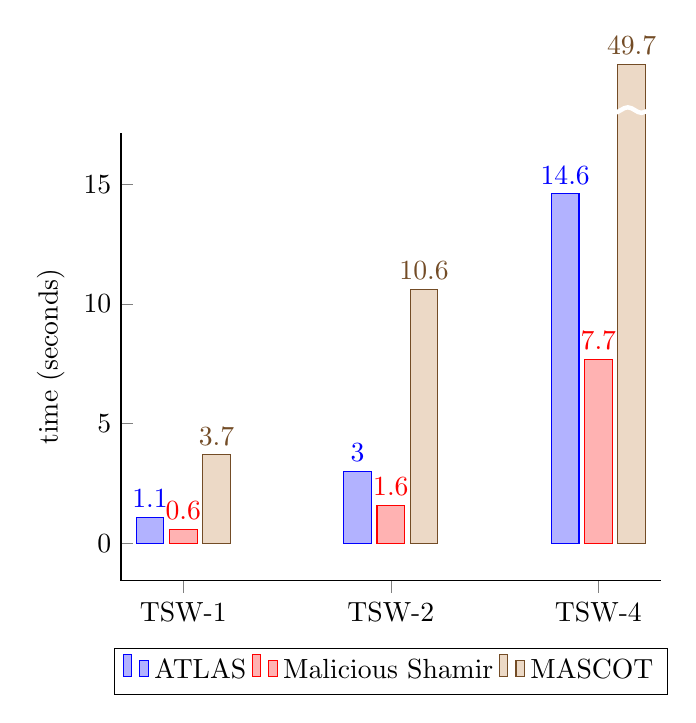
\begin{tikzpicture}
\begin{axis}[
    ybar,
    ymax=15,
    enlargelimits=0.15,
    legend style={at={(0.5,-0.15)},
      anchor=north,legend columns=-1},
    ylabel={time (seconds)},
    symbolic x coords={TSW-1,TSW-2,TSW-4},
    xtick=data,
    restrict y to domain*=0:20, % Cut values off at 20
    visualization depends on=rawy\as\rawy, % Save the unclipped values
    after end axis/.code={ % Draw line indicating break
            \draw [ultra thick, white, decoration={snake, amplitude=1pt}, decorate] (rel axis cs:0,1.05) -- (rel axis cs:1,1.05);
        },
    nodes near coords={%
            \pgfmathprintnumber{\rawy}% Print unclipped values
        },
    nodes near coords align={vertical},
    axis lines*=left,
    clip=false
    ]
\addplot coordinates {(TSW-1,1.1) (TSW-2,3) (TSW-4,14.6)};
\addplot coordinates {(TSW-1,0.6) (TSW-2,1.6) (TSW-4,7.7)};
\addplot coordinates {(TSW-1,3.7) (TSW-2,10.6) (TSW-4,49.7)};
\legend{ATLAS, Malicious Shamir, MASCOT}
\end{axis}
\end{tikzpicture}
\caption{Benchmark results for hash chains calculations over MPC (offline phase only) to sign a single message. Timing results are averaged over 10 runs in a network with 30ms delay.}
\end{figure}